\begin{figure}[hbtp]
  \centering
  % \subfigure[Naive-dynamic (ND) approach]{
  %   \label{fig:about-cases--naive}
  %   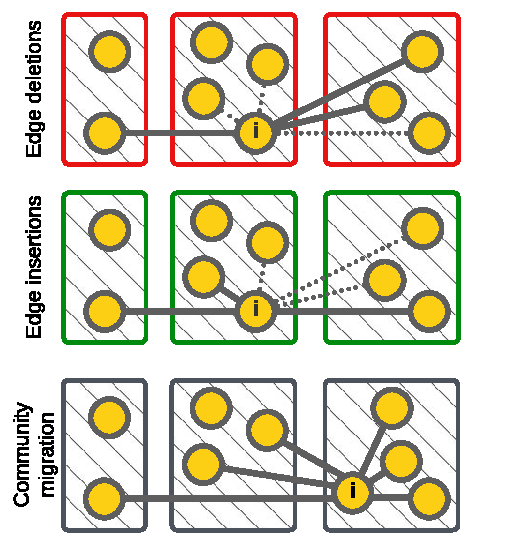
\includegraphics[width=0.3\linewidth]{out/about-cases-naive.pdf}
  % }
  \subfigure[Delta-screening (DS)]{
    \label{fig:about-cases--delta}
    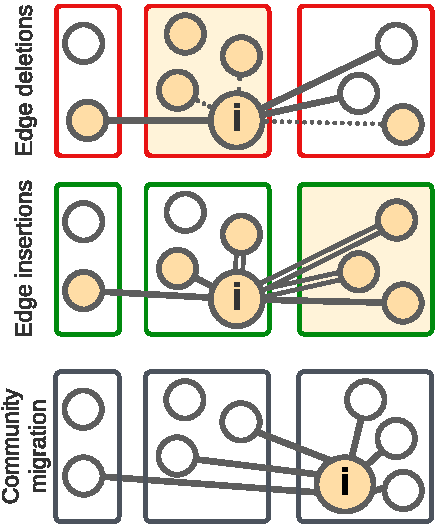
\includegraphics[width=0.468\linewidth]{out/about-cases-delta.pdf}
  }
  \subfigure[Dynamic Frontier (DF)]{
    \label{fig:about-cases--frontier}
    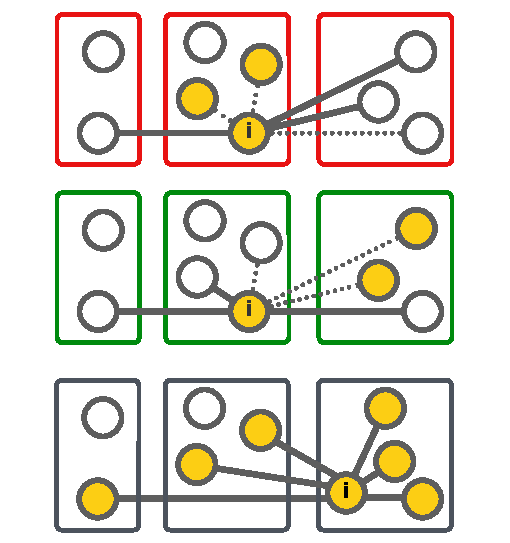
\includegraphics[width=0.43\linewidth]{out/about-cases-frontier.pdf}
  } \\[-1ex]
  \caption{Illustration of \textit{Delta-screening (DS)} \cite{com-zarayeneh21} and \textit{Dynamic Frontier (DF)} approaches \cite{sahu2024shared}, in the presence of edge deletions and insertions, represented with dotted lines and doubled lines, respectively. Vertices identified as affected (initial) by each approach are highlighted in brown, and entire communities marked as affected are depicted in light brown.}
  \label{fig:about-cases}
\end{figure}
